\documentclass[11pt]{article}
\usepackage[utf8]{inputenc}
\usepackage[spanish]{babel}
\usepackage{booktabs}
\usepackage{graphicx}
\usepackage{geometry}
\usepackage{hyperref}
\usepackage{caption}
\usepackage{enumitem}
\usepackage{amssymb}
\usepackage{xcolor}
\usepackage{tcolorbox}
\tcbuselibrary{skins,breakable}
\geometry{margin=2.2cm}

\definecolor{marcador}{RGB}{220,30,30}
\definecolor{decir}{RGB}{240,246,255}
\definecolor{decirborde}{RGB}{70,110,180}
\definecolor{hacer}{RGB}{255,246,230}
\definecolor{hacerborde}{RGB}{200,140,30}

\newtcolorbox{decirbox}{colback=decir, colframe=decirborde, boxrule=0.6pt, arc=2pt, left=6pt, right=6pt, top=4pt, bottom=4pt, breakable}
\newtcolorbox{hacerbox}{colback=hacer, colframe=hacerborde, boxrule=0.6pt, arc=2pt, left=6pt, right=6pt, top=4pt, bottom=4pt, breakable}

\title{Guion detallado del video de presentación\\
\large HW\_02\_202602 --- Acceso a salud resolutiva en Perú}
\author{Henry Llupton Capunay}
\date{\today}

\begin{document}
\maketitle

\begin{tcolorbox}[colback=gray!8, colframe=gray!50, arc=2pt]
\textbf{Duración objetivo: 11:30--11:50 (máximo 12:00, issue \#186).}
Cada bloque trae su minuto de inicio acumulado. Las cajas \textcolor{decirborde}{\textbf{azules ``Decir''}} son sugerencias de frase --- dilas con tus palabras, no las leas literal. Las cajas \textcolor{hacerborde}{\textbf{naranjas ``Hacer''}} son la acción física/de pantalla que acompaña. Antes de grabar: \texttt{streamlit run app.py} ya cargado en una pestaña (sin que se vea el tiempo de carga en cámara), y \texttt{report/main.pdf} a la mano.
\end{tcolorbox}

\tableofcontents
\vspace{0.3cm}

\section{Minutaje resumen}

\begin{center}
\begin{tabular}{lll}
\toprule
\textbf{Bloque} & \textbf{Inicio} & \textbf{Duración} \\
\midrule
1. Planteamiento y relevancia & 0:00 & 0:45 \\
2. Datos y problemas detectados & 0:45 & 1:30 \\
3. Método, engine y parámetros & 2:15 & 1:30 \\
4. Tres decisiones técnicas defendidas & 3:45 & 1:45 \\
5. Obstáculo, diagnóstico y solución & 5:30 & 2:00 \\
6. Demo en vivo del dashboard & 7:30 & 2:45 \\
7. Números y hallazgo central & 10:15 & 0:45 \\
8. Limitaciones & 11:00 & 0:30 \\
9. Cierre & 11:30 & 0:20 \\
\midrule
\textbf{Total} & & \textbf{11:50} \\
\bottomrule
\end{tabular}
\end{center}

\section{Bloque 1 --- Planteamiento y relevancia (0:00--0:45)}

\begin{decirbox}
``¿Cuánto tiempo tarda, por carretera, la población de un departamento
peruano en llegar a un establecimiento de salud con capacidad
\textbf{resolutiva} --- con quirófano, con capacidad de atender una
cesárea? La categoría de un establecimiento, de I-1 a III-E, determina
qué puede resolver in situ. La diferencia entre un puesto de salud sin
internamiento y un hospital II-1 puede ser la diferencia entre una
emergencia obstétrica atendida y una referida --- con el tiempo de
traslado como variable crítica.''

``Analicé tres departamentos elegidos para maximizar el contraste
geográfico: Tumbes en la costa, con red vial densa; Huancavelica en la
sierra, con altitud variable; y Madre de Dios en la selva, con red vial
dispersa.''

``Mi hipótesis de partida era que la dispersión de la red vial amazónica
penalizaría más el acceso que la topografía andina. Se las adelanto: se
confirma, pero no por la razón que yo esperaba --- eso lo cuento en el
minuto 10.''
\end{decirbox}

\begin{hacerbox}
Cámara a ti, sin pantalla compartida todavía. Habla con seguridad, es tu
apertura --- no hace falta mostrar nada en pantalla en este bloque.
\end{hacerbox}

\section{Bloque 2 --- Datos y problemas detectados (0:45--2:15)}

\begin{decirbox}
Recorre las 5 fuentes \textbf{rápido} (no más de 15-18s cada una):

``RENIPRESS de SUSALUD: 26,850 establecimientos a nivel nacional. El 26\,\%
no tiene coordenadas --- los descarté, documentado.''

``Para centros poblados, el issue sugería MINEDU/SIGMED, pero es un
geoportal interactivo sin descarga programática. Usé en su lugar el
shapefile oficial de Centros Poblados del IGN --- misma finalidad, mismo
portal de datos abiertos del Estado. Es una sustitución justificada, no
una desviación silenciosa.''

``Para población, no existe un CSV oficial por centro poblado --- usé la
población distrital de RENIEC, repartida por tipo de asentamiento.''

``Los polígonos distritales son el mismo shapefile del INEI que usa la
sesión 6 del curso para su choropleth.''

``Y la red vial: el extracto \texttt{peru-latest.osm.pbf} de Geofabrik ---
la fuente que el issue pide literalmente.''

\textbf{El hallazgo más revelador de esta fase (dilo con seguridad, es
evidencia de que investigaste de verdad):} ``el 53\,\% de los 136,587
centros poblados del IGN a nivel nacional no tiene código oficial. Usar
ese código como llave única colapsaba todos los nulos en un solo id
falso, y mi regla de duplicados los eliminaba como si fueran el mismo
registro. Uso \texttt{OBJECTID}, el id de fila del shapefile, en su
lugar.''
\end{decirbox}

\begin{hacerbox}
Comparte pantalla. Mientras hablas de las fuentes, ten \texttt{config.md}
o el navegador con los portales de datos abiertos abiertos de fondo (no
hace falta detenerte en ninguno). En el segundo 60 aprox., cambia al
dashboard y baja hasta el panel \textbf{``Calidad de datos (Fase 1)''}
(al final de la página) --- expande el expander \texttt{costa\_demanda}
2-3 segundos para que se vea la tabla de las 6 reglas con números reales,
y ciérralo. No te quedes ahí, es solo para probar que existe.
\end{hacerbox}

\section{Bloque 3 --- Método, engine y parámetros (2:15--3:45)}

\begin{decirbox}
``El motor es OSMnx más NetworkX, con un grafo \textbf{por departamento},
no nacional. Para tres departamentos chicos, un grafo nacional es más
lento de construir y cachear que tres grafos locales, y OSRM-Docker ---
la opción que recomienda el issue --- exige infraestructura que no se
justifica para este alcance.''

``Cada punto de demanda o facility se asigna al nodo más cercano del
grafo, con la distancia calculada en la zona UTM real del departamento
--- no con la aproximación de `1 grado igual a 111 kilómetros', que
ignora que un grado de longitud se encoge con el coseno de la latitud.''

``La matriz origen por facility invierte el problema: en vez de correr
Dijkstra desde cada punto de demanda, que son más numerosos, corro un
Dijkstra multi-fuente desde cada facility, sobre el grafo reversado ---
así el resultado sigue siendo el tiempo demanda-hacia-facility, aunque la
red tenga calles de un solo sentido.''

\textbf{El fallback (explícito, el issue lo pide literal):} ``Un punto
puede quedar en un componente vial desconectado de toda facility. En vez
de dejarlo indefinido, lo estimo vía distancia en línea recta a la
facility más cercana, multiplicada por un factor de desvío empírico ---
la mediana, por departamento, de tiempo real de red dividido tiempo de la
distancia recta a 30 kilómetros por hora. El factor sale distinto por
departamento: 0.80 en Tumbes, 1.07 en Huancavelica, 0.77 en Madre de
Dios. Que salga por debajo de 1 en costa y selva no es un error: la red
real, con tramos troncales a 60 u 100 kilómetros por hora, es en
promedio más rápida que una línea recta viajada a 30 parejos. Solo en la
sierra, con curvas y pendientes, ese efecto no alcanza a compensar.''
\end{decirbox}

\begin{hacerbox}
Muestra 3-4 segundos la Tabla 1 de \texttt{report/main.pdf} (``Fuente del
grafo de ruteo por departamento y perfil'') --- las 9 celdas dicen
\texttt{OSM (.pbf)}. Puedes tenerla ya abierta en una pestaña de PDF para
no perder tiempo buscando.
\end{hacerbox}

\section{Bloque 4 --- Tres decisiones técnicas defendidas (3:45--5:30)}

El issue pide \textbf{tres} decisiones técnicas explícitas, cada una con
la alternativa que descartaste y por qué. Estas son las tres más
defendibles del proyecto:

\begin{decirbox}
\textbf{(1) UTM dinámico por departamento, vs.\ el EPSG:24891 que usa la
sesión 6/7 del curso.}

``La clase usa EPSG:24891, PSAD56 zona oeste del Perú, para reproyectar a
nivel nacional en un panel de luces nocturnas --- razonable ahí, un CRS
`suficientemente bueno' alcanza para una variable de control de área. Pero
verifiqué con \texttt{pyproj} que ese CRS solo es válido al oeste de
79 grados oeste, la franja costera norte --- Huancavelica y Madre de Dios
caen fuera. Usé la zona UTM real de cada departamento en su lugar, al
costo de no poder sumar áreas directamente entre departamentos de zonas
distintas sin reproyectar antes --- no es un problema aquí porque cada
departamento se procesa por separado.''

\textbf{(2) El extracto \texttt{.osm.pbf} local vía pyrosm, vs.\ Overpass
API en vivo.} ``La decisión completa, con el diagnóstico paso a paso, va
en el siguiente bloque --- es la historia más importante del proyecto.''

\textbf{(3) Fallback con factor de desvío empírico, vs.\ dejar
\texttt{t\_min} indefinido.} ``Mi primera versión dejaba esos puntos como
valor nulo --- es lo más honesto en un sentido, y de hecho fue lo que
hice primero. Pero el issue pide explícitamente un fallback documentado
con un factor de desvío justificado, así que implementé la estimación y
la marqué con una columna booleana, \texttt{t\_min\_estimado}, para que
sea auditable cuál valor es medido y cuál estimado. No se pierde la
honestidad, se gana cumplimiento con lo que pide el issue.''
\end{decirbox}

\section{Bloque 5 --- Obstáculo, diagnóstico y solución (5:30--7:30)}

\textbf{Esta es la parte que más pesa en ``defensa de metodología''.
Cuéntala como una historia de detective, con ritmo, no como una lista de
hechos.} Tiene dos episodios reales, encadenados.

\begin{decirbox}
\textbf{Episodio A --- Overpass corta la conexión a los \textasciitilde
60 segundos.}

``Mi primera versión usaba la API Overpass en vivo. Departamentos chicos
como Tumbes completaban sin problema, pero Huancavelica --- 13 veces el
área máxima de consulta recomendada --- y Madre de Dios --- 67 veces ---
fallaban de forma intermitente. Primero sospeché que Overpass estaba
caído: falso, \texttt{/api/status} respondía 200 siempre. Después
sospeché que mi timeout de 10 segundos era muy corto: lo subí a 240,
mejoró parcialmente pero no de forma confiable. La pista real: los
fallos decían \texttt{Connection reset by peer} a intervalos casi
idénticos, 60 a 63 segundos, sin importar el timeout que yo configurara.
La conclusión: algo en la red de mi entorno de desarrollo corta las
conexiones salientes de larga duración a los 60 segundos --- un límite
externo, no del servidor Overpass ni de mi código. Solución: dejar de
depender de muchas peticiones cortas a una API remota, y procesar el
extracto \texttt{.osm.pbf} completo de forma local.''

\textbf{Episodio B --- el bug que se escondía detrás del primero (el más
fuerte de todo el proyecto, no lo apures, tómate 45--50 segundos).}

``Con el \texttt{.pbf} local, Madre de Dios mostraba una distancia de
snap de 131.8 kilómetros en promedio --- facilities aparentemente a 189
kilómetros de la demanda más cercana. Mi primera hipótesis: `OpenStreetMap
no tiene vías mapeadas en la selva profunda' --- sonaba plausible.
\textbf{Era la hipótesis equivocada.} Instrumenté el código paso a paso y
encontré que la función que arma el grafo sí traía la cobertura
completa: 665 mil nodos, hasta el borde real del área del departamento.
El recorte pasaba un paso después, en la función que convierte esos
datos a un grafo de red, cuyo parámetro \texttt{retain\_all} es falso por
defecto: descarta todo componente vial que no sea el más grande. La red
transitable de Madre de Dios resultó estar fragmentada en 313,529
componentes conexos --- el grafo cargado en memoria simplemente ya no
tenía la mitad del departamento, aunque el archivo fuente sí. Con ese
parámetro corregido, el snap bajó a 3.4 kilómetros, del mismo orden que
los otros dos departamentos.''

\textbf{Cierre del bloque, la lección meta --- dila, muestra criterio:}
``Los dos episodios comparten un patrón: el síntoma parecía apuntar a un
problema de datos --- `Overpass caído', `sin vías mapeadas' --- pero la
causa real estaba en el comportamiento por defecto de una librería.
Verificar antes de aceptar la explicación más fácil me tomó tiempo
extra, pero me evitó publicar un reporte con una conclusión geográfica
completamente al revés.''
\end{decirbox}

\begin{hacerbox}
No necesitas pantalla compartida en este bloque --- es el más narrativo
del video, la cámara sostenida en ti funciona mejor que texto en
pantalla. Si prefieres apoyo visual, ten el archivo
\texttt{src/routing.py} abierto en el fragmento del comentario sobre
\texttt{retain\_all} (busca ``La poda de componentes'' en
\texttt{report/main.tex} si quieres leer la cifra exacta en cámara).
\end{hacerbox}

\clearpage
\section{Bloque 6 --- Demo en vivo del dashboard (7:30--10:15)}

\textbf{Vale 2.5 de los 8 puntos del video --- es el bloque más largo a
propósito.} Antes de grabar: \texttt{streamlit run app.py} ya cargado,
sin spinner en cámara. Sigue el orden exacto de las capturas: cada
número rojo en la imagen es lo que señalas mientras dices la frase con
el mismo número.

\subsection*{6.1 --- KPI header, mapa e histograma (\textasciitilde 45s)}

\begin{figure}[h]
\centering
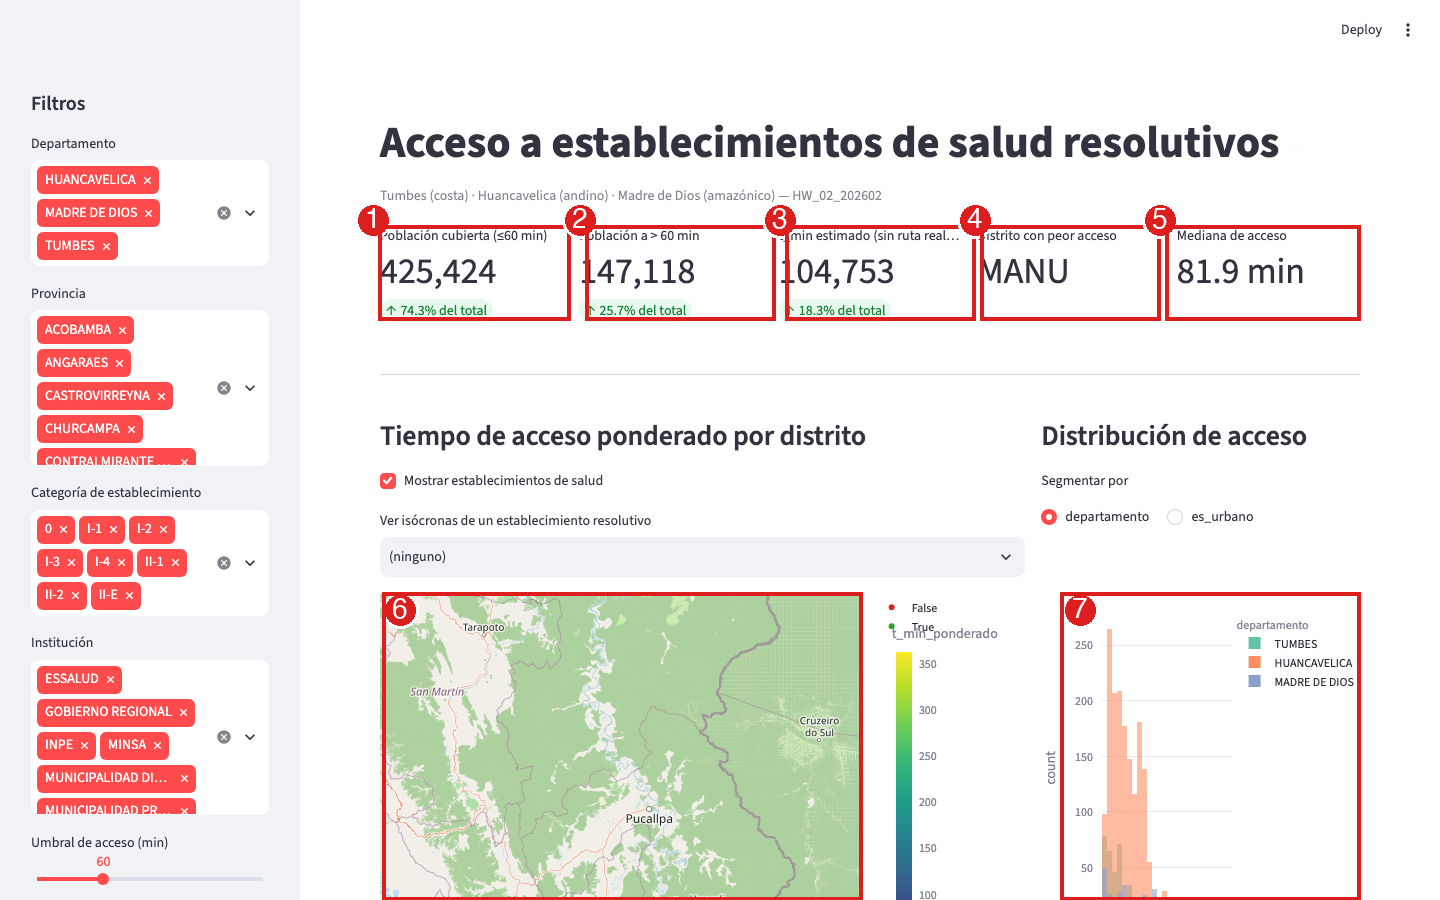
\includegraphics[width=0.97\textwidth]{video_assets/dash_1_top_annot.png}
\end{figure}

\begin{decirbox}
\textbf{1--5, KPIs (señala cada número de izquierda a derecha, 3-4s
cada uno):} ``Arriba tengo cinco indicadores: población cubierta dentro
del umbral que elija el usuario, población a más de 60 minutos, la
población cuyo \texttt{t\_min} viene del fallback por factor de desvío
--- una métrica nueva que agregué para que esa estimación no se pierda
entre los números medidos ---, el distrito con peor acceso, y la
mediana.''

\textbf{6, mapa:} ``El mapa colorea por tiempo de acceso ponderado ---
\emph{(en el sidebar, quita y vuelve a poner el filtro `Madre de Dios')}
--- y se actualiza en vivo con los filtros del panel izquierdo.''

\textbf{7, histograma:} ``Y acá la distribución de tiempos por
departamento, para ver la forma completa, no solo el promedio.''
\end{decirbox}

\begin{hacerbox}
En el sidebar (parte izquierda, fuera de esta captura): desmarca
``Madre de Dios'' del filtro Departamento y vuelve a marcarlo --- verás
el mapa y el histograma actualizarse solos. Después marca/desmarca el
checkbox ``Mostrar establecimientos de salud'' sobre el mapa. Si tienes
tiempo, abre el selectbox ``Ver isócronas de un establecimiento
resolutivo'' y elige uno --- aparecen los 3 anillos de color (30/60/120
min) sobre el mapa.
\end{hacerbox}

\subsection*{6.2 --- Tabla de distritos críticos (\textasciitilde 25s)}

\begin{figure}[h]
\centering
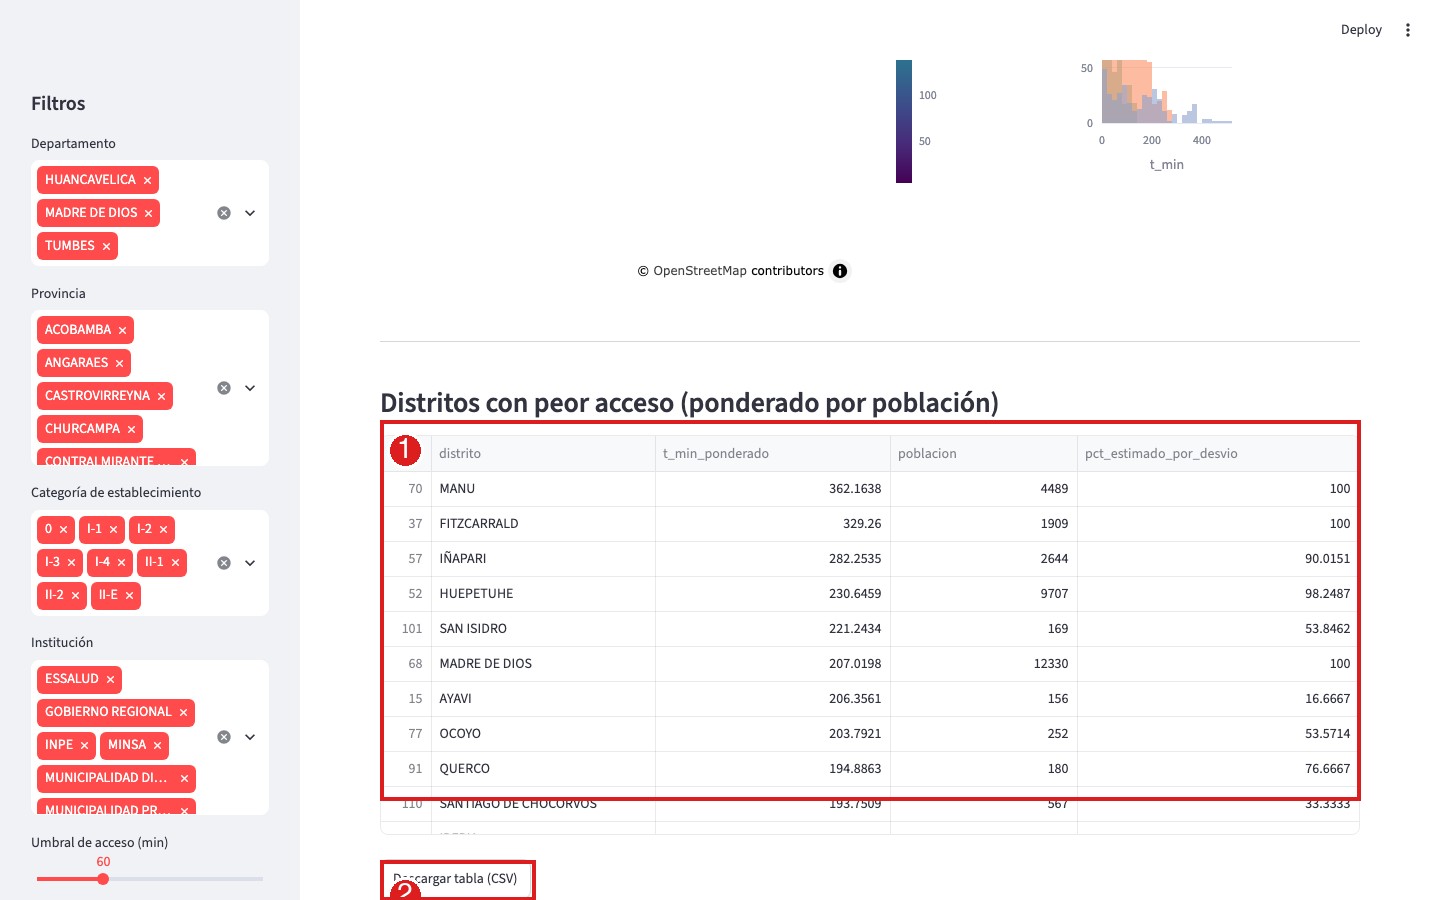
\includegraphics[width=0.97\textwidth]{video_assets/dash_2_criticos_annot.png}
\end{figure}

\begin{decirbox}
\textbf{1, tabla:} ``Esta es la tabla completa, ordenada, de distritos
con peor acceso ponderado por población --- con la columna
\texttt{pct\_estimado\_por\_desvio} al lado de cada uno, para auditar
cuánto de ese número es una ruta medida y cuánto una estimación.''

\textbf{2, botón:} ``Y se descarga en un clic, como pide el issue.''
\end{decirbox}

\begin{hacerbox}
Haz clic en el botón \textbf{``Descargar tabla (CSV)''} en cámara --- un
clic simple, se ve el archivo descargarse en la esquina del navegador.
\end{hacerbox}

\clearpage
\subsection*{6.3 --- El simulador de escenario (\textasciitilde 45s, la parte que más puntos vale)}

\begin{figure}[h]
\centering
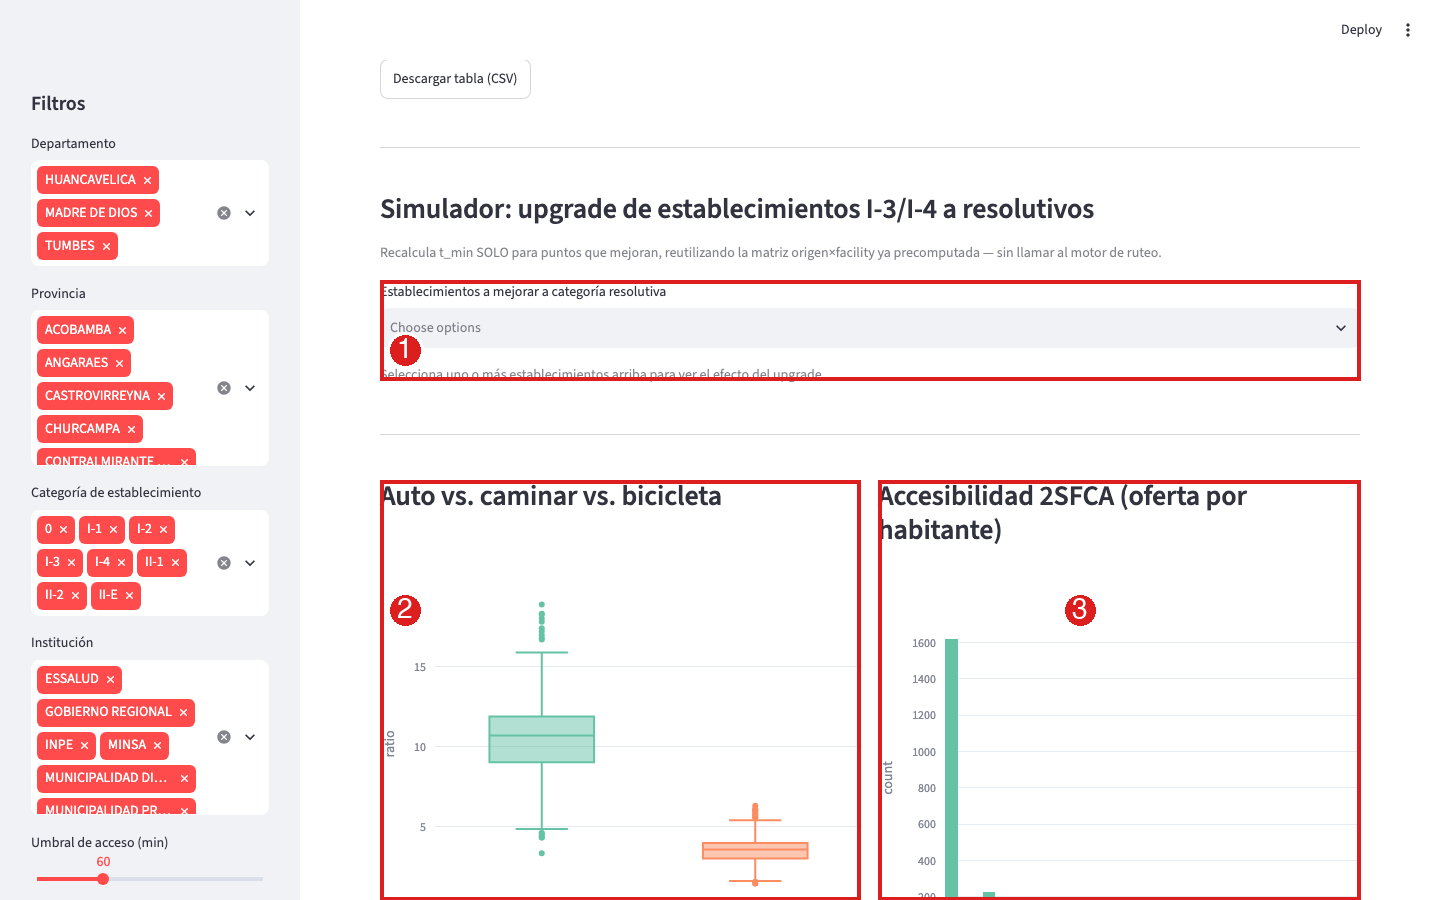
\includegraphics[width=0.97\textwidth]{video_assets/dash_3_simulador_annot.png}
\end{figure}

\begin{decirbox}
\textbf{1, simulador:} ``Y esta es la parte que más quiero mostrar: el
simulador de escenario. Selecciono uno o dos establecimientos categoría
I-3 o I-4 de Madre de Dios \emph{(ábrelo y elige mientras hablas)} y el
dashboard recalcula, al instante, cuánta población mejora su acceso si
esos establecimientos se convierten en resolutivos. Esto reutiliza la
matriz origen por facility ya precomputada --- no llama al motor de
ruteo, por eso es instantáneo. Miren la métrica y la tabla aparecer.''

\textbf{2, comparación de modos:} ``Acá la comparación auto, caminar y
bicicleta --- un hallazgo que no esperaba: Madre de Dios tiene el ratio
caminar-sobre-auto más \emph{bajo} de los tres departamentos, no el más
alto como hubiera supuesto para la selva.''

\textbf{3, 2SFCA:} ``Y la innovación 2: accesibilidad ponderada por
capacidad de oferta. La mediana es cero --- la mayoría de puntos de
demanda no tiene ninguna facility resolutiva dentro del umbral de 60
minutos, consistente con la escasez de oferta que ya vimos en Madre de
Dios.''
\end{decirbox}

\begin{hacerbox}
Abre el multiselect ``Establecimientos a mejorar a categoría
resolutiva'', elige 1 o 2 de la lista (busca los que digan Madre de
Dios en el nombre si se distinguen) --- espera 1-2 segundos a que
aparezca la métrica ``Población que mejora su acceso'' y la tabla
debajo, y señálalas. Este es el momento más importante de la demo, no
lo apures.
\end{hacerbox}

\subsection*{6.4 --- Panel de calidad de datos (\textasciitilde 15s, cierre de la demo)}

\begin{figure}[h]
\centering
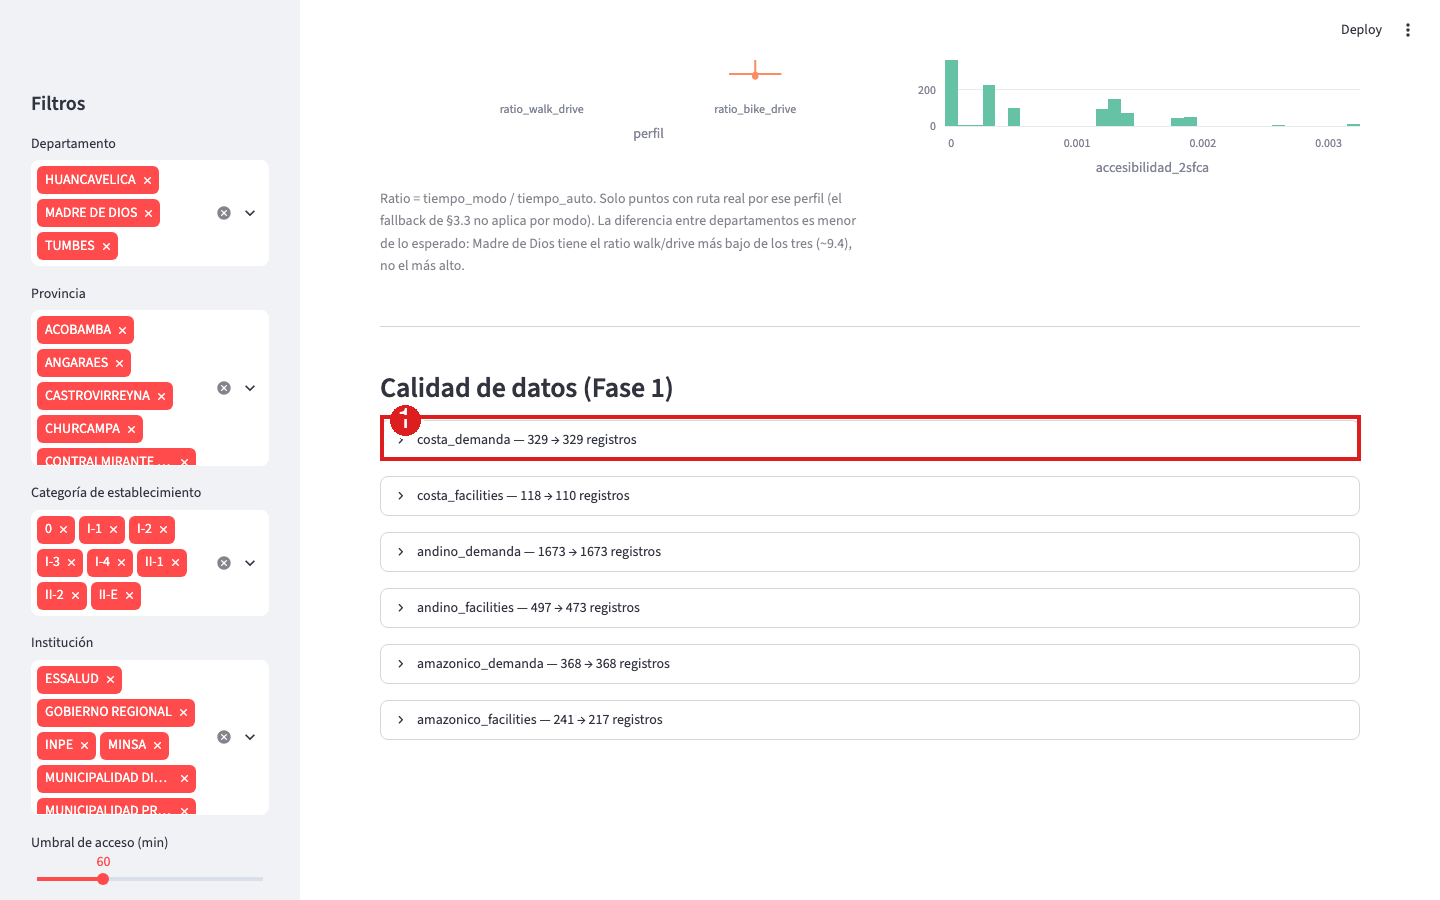
\includegraphics[width=0.97\textwidth]{video_assets/dash_4_calidad_annot.png}
\end{figure}

\begin{decirbox}
\textbf{1, panel:} ``Y al final, el panel de calidad de datos de Fase 1
--- cada expander trae el detalle de las 6 reglas de validación
obligatorias, con números reales, no simulados.''
\end{decirbox}

\begin{hacerbox}
Ya lo mostraste brevemente en el Bloque 2 --- acá solo un vistazo final
de 2-3 segundos para cerrar el recorrido del dashboard, no repitas la
explicación completa.
\end{hacerbox}

\clearpage
\section{Bloque 7 --- Números y hallazgo central (10:15--11:00)}

\begin{decirbox}
\textbf{El clímax del video --- números exactos, sin titubear:}

``Con red vial real y completa, y el fallback aplicado, mi hipótesis de
partida \textbf{se confirma}: Madre de Dios tiene el peor acceso
ponderado de los tres departamentos --- \textbf{87.3 minutos}, frente a
51.4 en Huancavelica y 14.4 en Tumbes. Pero el mecanismo no es el obvio.
Entre población con ruta real, los tiempos son parecidos: alrededor de
48 a 51 minutos en ambas geografías peor conectadas --- Huancavelica no
gana en velocidad. Lo que separa a Madre de Dios es que \textbf{35.7\,\%
de su población no tiene ninguna ruta vial mapeada} a una facility
resolutiva --- casi 4 veces la tasa de Huancavelica, que es 9.2\,\%. Es
una falla de \textbf{conexión}, no de \textbf{velocidad de trayecto}.''

``Otros números: el Gini ponderado es 0.67. Madre de Dios tiene solo
\textbf{2} establecimientos resolutivos activos en todo el
departamento --- lo verifiqué de forma independiente contra el CSV
crudo de RENIPRESS. Y la comparación línea recta contra red: en
Huancavelica, ignorar la red vial le cuesta a la población conectada una
mediana de \textbf{13.4 minutos} adicionales --- la evidencia mecánica de
que ahí el problema es topografía, no ausencia de ruta.''

\textbf{Recomendaciones (elige 2, no leas las 5 del reporte):}

``Recomiendo, primero, verificar contra imágenes satelitales si los
313,529 componentes fragmentados de Madre de Dios son tramos físicamente
inconexos o vacíos de etiquetado en OpenStreetMap. Y segundo, priorizar
intervención vial de velocidad --- no de conexión --- en los distritos
críticos de Huancavelica, porque ahí el cuello de botella es
demostrablemente el trayecto.''
\end{decirbox}

\section{Bloque 8 --- Limitaciones (11:00--11:30)}

\begin{decirbox}
No las leas todas --- elige 2 y dilas con seguridad, no a la carrera
como quien se disculpa:

``El \texttt{t\_min} de los puntos sin ruta real es una
\textbf{estimación}, no una medición --- más incertidumbre que un punto
con ruta real, y está marcado explícitamente para que se pueda
auditar.''

``No integré una fuente de altitud real --- el cross-analysis
correspondiente reporta honestamente \texttt{n=0} en vez de inventar
una correlación.''
\end{decirbox}

\section{Bloque 9 --- Cierre (11:30--11:50)}

\begin{decirbox}
``El pipeline completo --- desde datos crudos hasta este dashboard ---
corre con un solo comando, \texttt{python run\_pipeline.py --real}, está
en el repositorio, y cada número que mostré hoy sale de ahí, no de una
hoja de cálculo aparte. Gracias.''
\end{decirbox}

\vspace{0.4cm}
\begin{tcolorbox}[colback=gray!8, colframe=gray!50, arc=2pt, coltitle=black, colbacktitle=gray!25, title=\textbf{Checklist final antes de exportar}]
\begin{itemize}[leftmargin=1.2em, itemsep=2pt]
\item[$\square$] Framing del problema + pipeline explicado (bloques 1--3)
\item[$\square$] Tres decisiones técnicas + obstáculo/diagnóstico/solución (bloques 4--5)
\item[$\square$] Demostración en vivo del dashboard, incluyendo el simulador (bloque 6)
\item[$\square$] Hallazgos, limitaciones y recomendaciones con números concretos (bloques 7--8)
\item[$\square$] Duración total $\le$ 12:00
\item[$\square$] Audio limpio, sin ruido de fondo; pantalla compartida legible (letra no muy chica)
\end{itemize}
\end{tcolorbox}

\end{document}
